\chapter{Suites géométriques}
\thispagestyle{fancy}

\section{Définition}

\begin{bexemple}
    Considérons une suite numérique $U_n$ où le rapport entre un terme et son précédent reste constant et égale à 2.\\
    Si le premier terme est égal à 5, les premiers termes successifs sont :\\
    $U_0 = 5$,\ \ \ 
    $U_1 = 10$,\ \ \ 
    $U_2 = 20$,\ \ \ 
    $U_3 = 40$.\\
    Une telle suite est appelée une suite géométrique de raison $2$ et de premier terme $5$.\\
    La suite est donc définie par : $U_{n+1}=2\times U_n$ et $U_0=5$. 
\end{bexemple}

\begin{bdefi}
    Une suite $U_n$ est une \grasInDef{suite géométrique} s'il existe un nombre q tel que pour tout entier $n$, on a : $U_{n+1}=q\times U_n$.
    Le nombre $q$ est appelé \grasInDef{raison} de la suite.
\end{bdefi}

\begin{bmethodet}{Démontrer si une suite est géométrique}
    La suite $U_n$ définie par : $U_n=3\times 5^n$  est-elle géométrique ?
    \ \\
    $\dfrac{U_{n+1}}{U_n} =\dfrac{3\times 5^{n+1}}{3\times 5^n}=\dfrac{5^{n+1}}{5^n} =5^{n+1-n}=5$\\
    Le rapport entre un terme et son précédent reste constant et égale à $5$.\\
    $U_n$ est une suite géométrique de raison $5$ et de premier terme $U_0=3\times 5^0=3$.
\end{bmethodet}

\begin{bexemplet}{exemple concret}
    On place un capital de \EUR{500} sur un compte dont les intérêts annuels s'élèvent à $4\%$.
    Chaque année, le capital est multiplié par $1,04$.
    Ce capital suit une progression géométrique de raison $1,04$.\\
    
    On a ainsi :\\ 
    $U_1=1,04\times 500=520$\\		
    $U_2=1,04\times 520=540,80$\\
    $U_3=1,04\times 540,80=562,432$\\	
    De manière générale : $U_{n+1}=1,04\times U_n$ avec $U_0=500$\\ 
    On peut également exprimer $U_n$ en fonction de $n$ : $U_n= 500\times1,04^n$. 
\end{bexemplet}

\begin{propriete}
    $U_n$ est une suite géométrique de raison $q$ et de premier terme $U_0$.\\
    Pour tout entier naturel $n$, on a : $U_n= U_0\times q^n$.
\end{propriete}

\begin{bdemo}
    La suite géométrique $U_n$ de raison $q$ et de premier terme $U_0$ vérifie la relation
    $U_{n+1}=q\times U_n$.
    \begin{itemDem}
    	\item Si $q$ ou $U_0$ est nul, alors tous les termes de la suite sont nuls. La démonstration est évidente dans ce cas.
    	\item Dans la suite, on suppose donc que $q$ et $U_0$ sont non nuls. Dans ce cas, tous les termes de la suite sont non nuls.
    \end{itemDem}
    En calculant les premiers termes :\\ 
    $U_1=q\times U_0$\\
    $U_2=q\times U_1$\\
    $U_3=q\times U_2$\\
    …\\
    $U_n=q\times U_{n-1}$\\
    \\
    En multipliant membre à membre ces $n$ égalités, on obtient :
    $u_1\times U_2\times U_3\times …\times U_n=U_0\times U_1\times U_2\times …\times u_{n-1}\times q^n$.\\
    Comme les termes de la suite sont non nuls, on peut diviser aux deux membres les facteurs identiques : $U_n=U_0\times q^n$
\end{bdemo}

\begin{bmethodet}{Déterminer la raison et le premier terme d'une suite géométrique}
Considérons la suite géométrique $U_n$ tel que $U_4=8$ et $U_7=512$.\\
Déterminer la raison et le premier terme de la suite $U_n$.\\
\\
\ \\
Les termes de la suite sont de la forme $U_n=U_0\times q^n$.\\
Donc : $U_4=U_0\times q^4=8$ et $U_7=U_0\times q^7=512$.\\
Ainsi : $\dfrac{U_7}{U_4}  = \dfrac{U_0\times q^7}{U_0\times q^4}  =q^3$ et $\dfrac{U_7}{U_4}=\dfrac{512}{8}=64$ donc $q^3=64$.\\
On utilise la fonction racine troisième de la calculatrice pour trouver le nombre qui élevé au cube donne 64.\\
Ainsi $q=^3\sqrt{64}=4$\\
Comme $U_0 \times q^4=8$, on a : $U_0\times 4^4=8$ et donc : $U_0= \dfrac{1}{32}$.
\end{bmethodet}

\section{Représentation graphique}

\begin{bexemple}
    La suite géométrique $U_n$ définie par $U_n=-4\times2^n$ est décroissante car le premier terme est négatif et la raison est supérieure à 1
    \begin{center}
        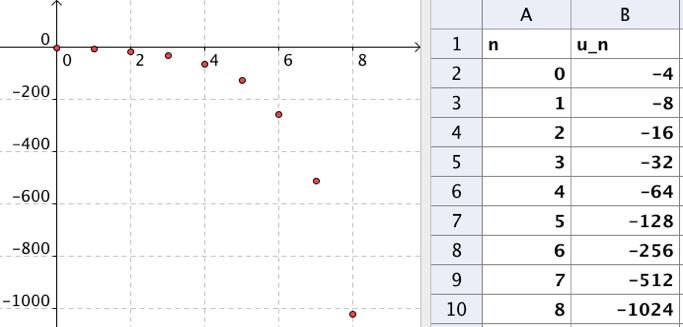
\includegraphics[scale=1]{01-07-03.png}
    \end{center}
    Remarque : Si la raison q est négative alors la suite géométrique n'est pas monotone.
\end{bexemple}
% \begin{center}
%     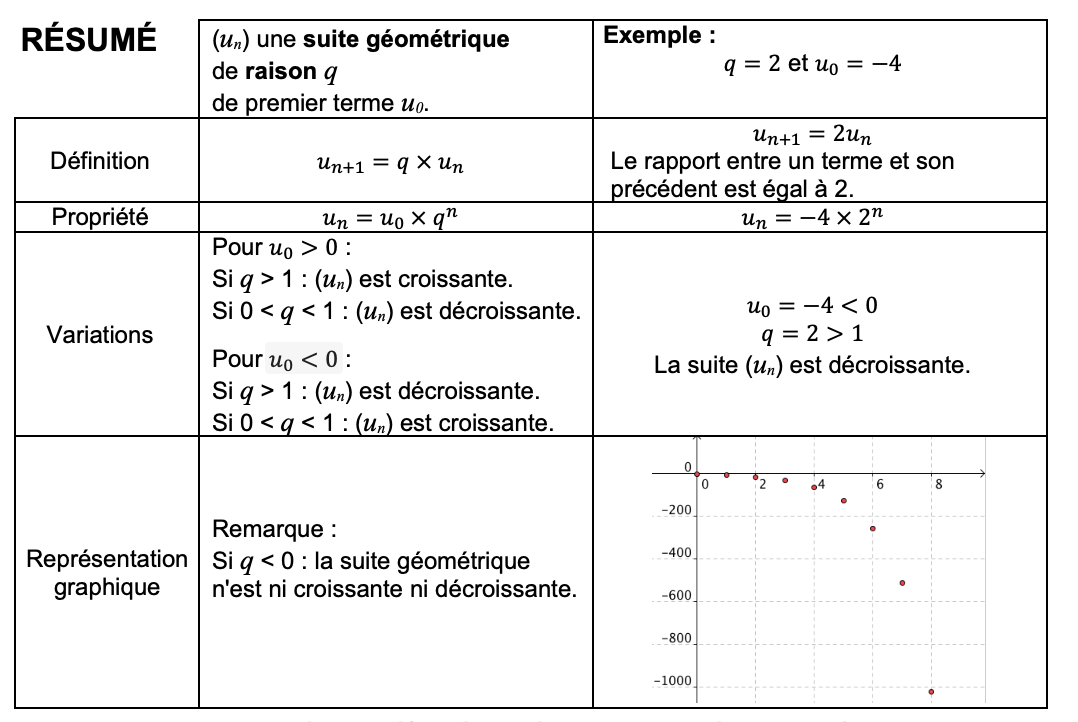
\includegraphics[scale=0.8]{01-07-04.png}
% \end{center}

\section{Somme des termes consécutifs d'une suite géométrique}

\subsection{Cas d'une suite géométrique}

\begin{bprop}
    $n$ est un entier naturel non nul et $q$ un réel différent de 1 alors on a :\\ 
    $1+q+q^2+q^3+...+q^n= \dfrac{1-q^{n+1}}{1-q}$
\end{bprop}

\begin{brmq}
    Il s'agit de la somme des $n+1$ premiers termes d'une suite géométrique de raison $q$ et de premier terme $1$.
\end{brmq}

\begin{bdemo}
    $S=1+q+q^2+q^3+...+q^n$\\
    $q\times S=q+q^2+q^3+q^4+...+q^(n+1)$\\
    \\
    Ainsi :\\
    $S-q\times S=(1+q+q^2+q^3+...+q^n )-(q+q^2+q^3+q^4+...+q^{n+1})$\\
    $S-q\times S=1-q^(n+1)$\\
    $S\times (1-q)=1-q^{n+1}$\\
    $S=\dfrac{1-q^(n+1)}{1-q}$
\end{bdemo}

\begin{bmethodet}{Calculer la somme des termes d'une suite arithmétique}
Calculer la somme $S$ suivante : 
$S=1+3+3^2+3^3+...+3^{13}$\\
\\
$S=1+3+3^2+3^3+...+3^{13}=\dfrac{1-3^{14}}{1-3}=2\  391\  484$

\end{bmethodet}


